\documentclass[a4paper]{article}

\usepackage[utf8]{inputenc}
\usepackage[T1]{fontenc}
\usepackage[francais]{babel}
\usepackage[top=2cm,bottom=2cm,left=3cm,right=2cm]{geometry}
\usepackage{setspace}
\usepackage{graphicx}

\title{Introduction à Git et à GitHub}
\author{Antoine \bsc{Wacheux}}
\date{30 mars 2013}

\onehalfspace

\begin{document}

\maketitle

Dans ce petit guide, vous trouverez toute les informations nécessaires pour utiliser efficacement git pour gérer des projets. Ce document est loin d'être exhaustif, beaucoup de notions avancées seront passées sous silence car elles sont trop compliquées pour être abordées dans le cadre d'une seule formation. Dans un première parti, je vous présenterai ce qu'est git et vous ferai un bref historique. Nous verrons également sont installation, ça configuration pour une mise en place rapide ainsi que les commandes de bases. Dans une seconde parti, je vous présenterai le site GitHub qui est l'un des plus grands hébergeur de dépôt git. Nous verrons comment créer notre propre dépôt, et comment participer à des projets existants. Enfin dans une troisième partis j'aborderai une notion délicate, la notion de branche. 

\paragraph{Remarque :} Ici, je n'aborderai l'utilisation de git que par la console. Des interfaces graphiques existent mais il est préférable de savoir utiliser version console au préalable car cela permet de comprendre exactement les différentes opérations qui sont effectuées et de dépanner plus facilement par la suite. 

\paragraph{Convention :} Voici les différentes conventions que j'utiliserai pour l'écriture des commandes dans un terminal : 

\begin{verbatim}
// Ceci est un commentaire
- # apt-get install git-core // Ceci est un commande à executer en tant que super-utilisateur 
(utiliser sudo)
- git commit -a //Si la commande est donnée telle quelle, elle doit être exécuté en tant 
qu'utilisateur normal
\end{verbatim}

\tableofcontents

\part{Les bases de Git}

\section{Introduction à Git}

\subsection{Présentation}

Git, prononcé “guite”, est un gestionnaire de version. C'est un logiciel qui permet d'enregistrer toutes les modifications apportées à un ensemble de fichiers. Ainsi il est très aisé de se \og balader dans le temps \fg pour revenir à des versions antérieures. Ce genre de logiciel est particulièrement utile pour la gestion de projet impliquant plusieurs personnes, car il permet de gérer automatiquement toutes les modifications apportées par l'ensemble de l'équipe et de maintenir une version à jour chez chacun de ses membres. Mais, c'est encore plus puissant, car il permet de très facilement identifier et de supprimer les modifications causant une instabilité dans le projet. Il est également très utile d'utiliser un gestionnaire de version sur un projet personnel, j'entends par-là un projet ou l'on est seul à travailler, car même sur ce genre de projet il peut être utile de revenir facilement à des versions plus stables, le tout sans risque de se tromper en enlevant les modifications.

Maintenant ce pose la question : Pourquoi Git ? En effet, il existe plusieurs gestionnaires de versions libre et gratuit autre que git. On peut ainsi citer Mercurial, Bazar ou Subversion. Eh bien Git possède plusieurs avantages. Le premier est qu'il s'agit d'un logiciel récent, il date de 2005. De ce fait il ne possède pas nombre des défauts de ses concurrents. Ensuite, il est rapide, bien plus rapide que Subversion ou CVS par exemple. Et il est décentralisé. C'est-à-dire qu'il n'a pas besoin d'un serveur central pour héberger le projet entier. Il est capable de se connecter à chaque ordinateur de chaque membre d'une équipe pour récupérer les dernières modifications. Cependant, nous l'utiliserons ici que de manière centralisée pour faciliter la gestion des projets.

\subsection{Un bref historique}

Git a été développé en 2005 pour les besoins du noyau Linux. A l'époque l'équipe du noyau utilisait le gestionnaire de version BitKeeper jusqu'à ce que celui-ci ne soit plus gratuit. L'équipe du noyau Linux a donc décidé de prendre les choses en main en développant son propre gestionnaire de version avec ces propres contraintes. Ce nouveau gestionnaire devait être :
\begin{itemize}

\item vitesse
\item conception simple
\item le support d'un nombre élevé de branches
\item complètement décentraliser
\item efficace dans la gestion de gros projet tant au niveau de la rapidité que de la compression des données

\end{itemize}

Depuis sa naissance, Git a évolué mais a su également conserver toutes ses qualités qui font de lui un excellent gestionnaire de version.

\section{Fonctionnement global de Git}

Git fonctionne par dépôt. Un dépôt est un ensemble de fichier qui sont suivis par Git. Voici à quoi ressemble un dépôt

\begin{verbatim}
ls -alh


total 216K
drwxr-xr-x 3 antoine ####### 4,0K 30 mars  17:50 .
drwxr-xr-x 3 antoine ####### 4,0K 30 mars  12:40 ..
drwxr-xr-x 8 antoine ####### 4,0K 30 mars  13:26 .git
-rw-r--r-- 1 antoine #######  211 30 mars  12:49 .gitignore
-rw-r--r-- 1 antoine #######  781 30 mars  17:50 poly_git.aux
-rw-r--r-- 1 antoine #######  18K 30 mars  17:50 poly_git.log
-rw-r--r-- 1 antoine ####### 143K 30 mars  17:50 poly_git.pdf
-rw-r--r-- 1 antoine #######  16K 30 mars  17:50 poly_git.synctex.gz
-rw-r--r-- 1 antoine ####### 5,0K 30 mars  17:50 poly_git.tex
-rw-r--r-- 1 antoine #######  446 30 mars  17:50 poly_git.toc
-rw-r--r-- 1 antoine #######   70 30 mars  12:49 README.md

\end{verbatim}

Tous les fichiers sont suivis par git. Chacune des modifications qui y sera faites sera automatiquement détectée. Quand les changements son jugés satisfaisants, on les sauvegardes. Git étant un logiciel intelligent, il ne va pas sauvegarder à chaque changement le fichier dans son intégralité, il va juste prendre les portions ont été modifiées, les empaqueter et les compresser. Le paquet ainsi créer s'appelle un commit. Ainsi la version actuel du dépôt correspond à la \og somme \fg des changements apportés par chaque commit.

\begin{figure}[h]
\centering
\label{figure_commit}
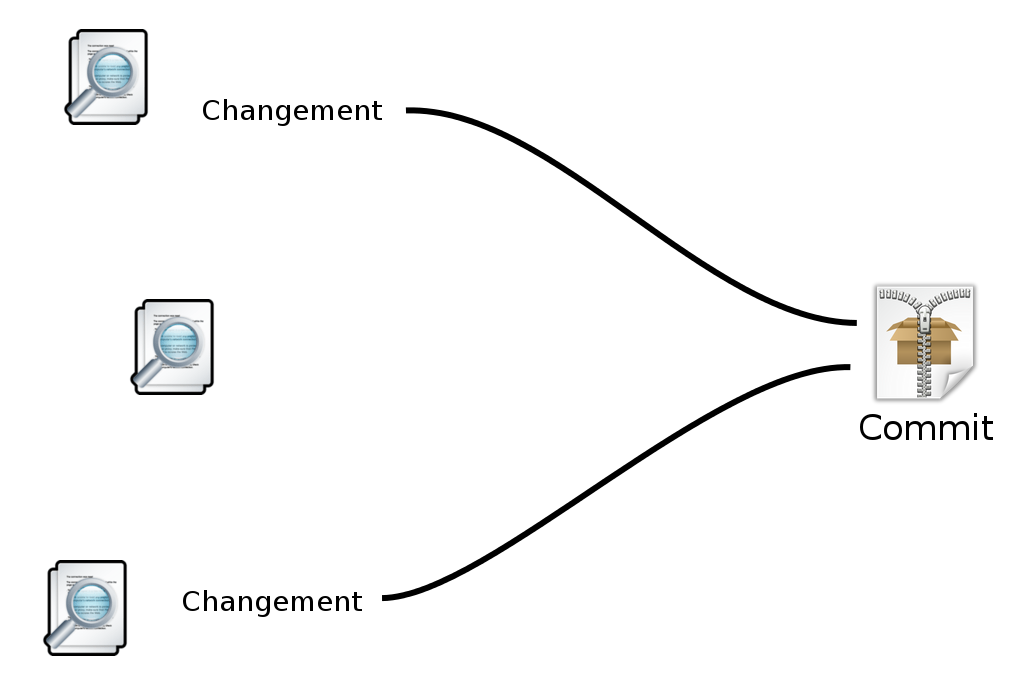
\includegraphics[scale=0.25]{commit.png}
\caption{Processus de création de commit}
\end{figure}

Ensuite chaque commit est envoyé vers le dépôt centrale, cette opération s'appelle la fusion. Chaque utilisateurs devra ensuite récupérer tout les commits envoyés et les fusionnés avec ça copie du dépôt. Si deux commits modifient la même partie d'un fichier, il y a ce que l'on appel un \textbf{conflit} et c'est à l'utilisateur de le résoudre en indiquant à Git qu'elle version garder.

Le répertoire \emph{.git} contient la liste de tout les commit, les configurations propres au dépôts, les branches, l'adresse du dépôt central. En gros, c'est ce qui permet à git de suivre correctement le projet, il convient donc de ne pas y toucher.

\end{document}